\section{Introduction}

Pour mon stage de fin de licence, j'avais un stage de 7~semaines a effectué en entreprise ou en laboratoire. En fonction de si l'on voulait s'insérer dans le monde professionnel ou académique. Pour ma part, car je souhaite  m'orienter vers un parcours professionnel, j'ai choisi de faire mon stage en entreprise à Orano. % en fonction de si l'on souhaite s'insérer dans le monde professionnel ou académique. Pour ma part, car je souhaite m'orienter vers un parcours professionnel, j'ai choisi de faire mon stage en entreprise à Orano.
\subsection{Orano}
Orano est un grand groupe français spécialisé dans le cycle du nucléaire. Elle dispose 17~500~collaborateurs repartie dans 17~pays et avait un revenu de 4,8~M€ en 2023~\cite{report:rapport_activiter}. Elle est née en 2018 à la suite d'une restructuration d'Areva. Elle est présente dans plusieurs domaines du nucléaire, de l'extraction de l'uranium à la gestion des déchets nucléaires en passant par la production de combustible. Ses différentes activités sont réparties dans plusieurs binuessus unit~:
\begin{description}
    \item [Orano Support] qui regroupe les activités de support du groupe
    \item [Orano Mining]qui regroupe les activités d'extraction d'uranium
    \item [Orano Medical]qui regroupe les activités de production de radioéléments pour la médecine nucléaire
    \item [Orano Batteries]qui regroupe les activités de recyclage de batterie
    \item [Orano Dismantling]qui regroupe les activités de démantèlement de centrale nucléaire
    \item [Orano Chimie-Enrichissement]qui regroupe les activités de chimie et d'enrichissement de l'uranium
\end{description}
\begin{figure}
    \centering
    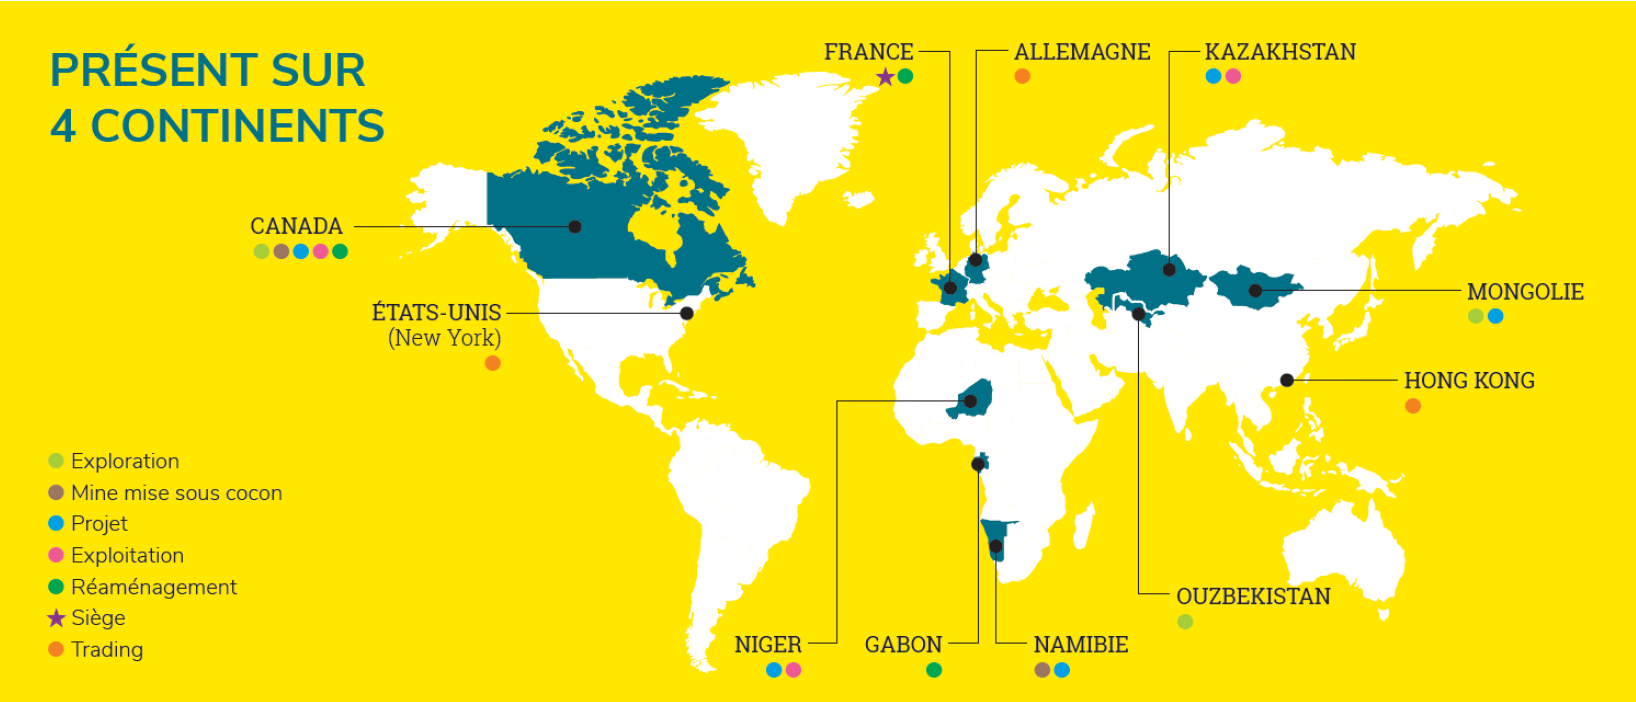
\includegraphics[width=\textwidth]{Carte-ornao-international.png}
    \caption[Carte des activités d’Orano dans le monde]{Carte des activités d’Orano dans le monde, Source~: Dossier d’information Orano~2020}
    \label{fig_carte_orano}
\end{figure}









Ces filiales sont présentes à l'international avec des mines d'uranium au Kazakhstan, au Canada et au Niger, de l'exploration ou des projets en Namibie, en Ouzbékistan et en Mongolie. La majorité des sites à l'étranger d'Orano sont des sites d'Orano Mining due à la nature de ses activités. C'est dans cette dernière que j'ai effectué mon stage.  %pas a la bonne place

\subsection{Orano Mining}

Orano mining est en charge de tout ce qui est relatif à l'extraction de l'uranium. Nous pouvons repartir ses activités en 4~grands domaines~:%remediation generation de nouveux projet et exploration. explo ,prod, projet, remediation (amf) %parler de nouveaux projet
\subsubsection{L'exploration}
L'exploration est la première étape de l'extraction de l'uranium. Elle consiste à trouver des gisements d'uranium. Pour cela, Orano Mining utilise des méthodes géophysiques et géochimiques pour trouver des gisements d'uranium. Une fois un gisement trouvé, il faut l'exploiter.

\subsubsection{L'exploitation}
L'exploitation est la deuxième étape de l'extraction de l'uranium. Elle consiste à extraire l'uranium du sol. Pour cela, Orano Mining utilise diverses méthodes d'extraction en fonction de la nature du gisement. On peut citer~:
\begin{description}
    \item [L'extraction in situ] qui consiste à injecter de l'acide dans le sol entre deux couches étanche pour dissoudre l'uranium et le remonter à la surface (voir \cref{ssec_insitu}). C'est le cas des mines de Muyunkum et Tortkuduk au Kazakhstan.
    \item [L'extraction par jetboring]qui consiste à creuser un trou dans le sol et à injecter de l'eau sous pression pour remonter l'uranium à la surface (voir \cref{ssec_jetbore}). C'est le cas de la mine Cigar Lake au Canada.
    \item [L'extraction à ciel ouvert]qui consiste à creuser une fosse pour extraire l'uranium. C'est le cas de la mine de Somaïr au Niger et de Mclean Lake au Canada (production suspendue entre 2008 et 2025 suite à la chute du cours de l'uranium).
\end{description}


\subsubsection{Le traitement}
\begin{wrapfigure}{r}{0.5\textwidth}
    \centering
    \href{https://commons.wikimedia.org/wiki/File:Yellow_Cake_Uranium_(14492248719).jpg}{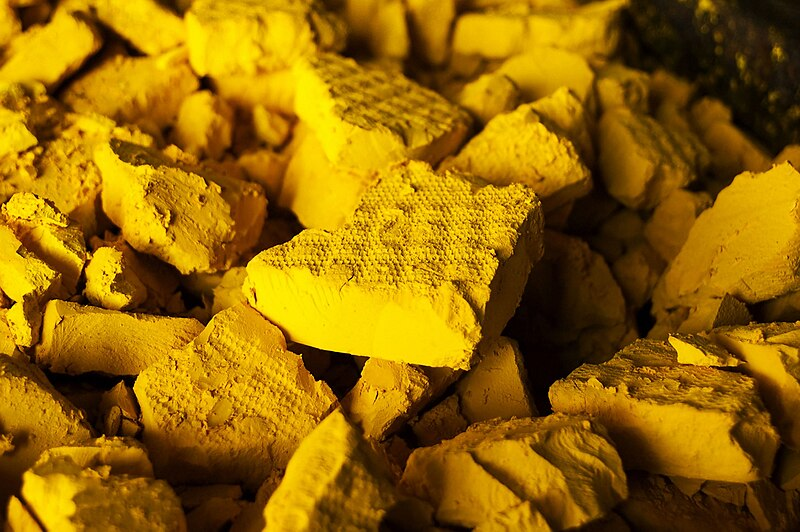
\includegraphics[width=0.5\textwidth]{Yellow_Cake_Uranium_(14492248719).jpg}}
    \caption[Apparence du yellow cake]{Apparence de yellow cake. Avec des méthodes modernes, certains traitements peuvent lui donner une apparence marron, voir noir. Source~: \href{https://commons.wikimedia.org/wiki/File:Yellow_Cake_Uranium_(14492248719).jpg}{Nuclear Regulatory Commission from US}, Public domain, via Wikimedia Commons}
    \label{fig_yellow-cake}
\end{wrapfigure}

Le traitement est la dernière étape de l'extraction de l'uranium. Elle consiste à traiter le minerai pour en extraire l'uranium. Pour cela, Orano Mining utilise des méthodes de traitement chimique pour extraire l'uranium du minerai. Généralement, cette étape est faite avec une lixiviation de l'uranium par une solution concentrée acidique, alcaline ou de peroxyde pour former ce que l'on appellera du "yellow cake" due à sa couleur et texture (voir \cref{fig_yellow-cake}). Le yellow cake est composer de 70~\% à 90~\% d'oxyde d'uranium notamment d'$U_3O_8$~\cite{article:composition-yellow-cake}. Une fois l'uranium extrait, il est envoyé à Orano Chimie-Enrichissement ou a d'autres partenaires pour être enrichi. En effet, l'uranium naturel est composé à 0,7~\% d'uranium~235 et a 99,3~\% d'uranium~238 avec une concentration moyenne de 2.7~ppm~\cite{site:natural_uranium}. Pour être utilisé dans un réacteur, il faut que l'uranium~235 soit enrichi entre 3~\% à 5~\% d'$U_{238}$~\cite{article:uranium-concentration}



\subsubsection{L'après-mine}
L'après-mine désigne l'ensemble des actions de remédiation et de monitoring qui sont entrepris par Orano après qu'une mine ferme. En effet, une fois une mine fermée, il faut la remettre en état pour éviter les risques de pollution. Pour cela, Orano Mining met en place des systèmes de monitoring pour surveiller l'évolution de la mine et des actions de remédiation pour remettre la mine en état. En France, Orano a la charge de 235 sur 247 des sites miniers d'uranium présent sur le territoire dont des sites qu'Orano n'a pas exploité~\cite{site:orano_apres_mine}. L'après-mine n'intervient pas qu'en France, mais aussi a l'étranger. Par exemple, au Canada, Orano a fini la remédiation de la mine de Cluff Lake (1979-2002) en 2013 et le site a été réouvert au public. En 2023, le gouvernement a été satisfait des actions d'Orano et les terres, on était rendu à l'état provincial~\cite{site:Cluff_lake_remediation}.

\subsection{Direction de la transformation digitale}
% fait partie des projet de la mine %pas petit 
Au sein de la mine est un petit service qui est en charge de la transformation digitale de la mine. Ce service est en charge de mettre en place divers outils digitaux pour acompagner %(les projet les expotation dans monde de demains). Il travaille en collaboration avec les différents services de la mine pour comprendre leur besoin et mettre en place des outils qui répondent à leur besoin. Par exemple, un des grands sujets étais la était la digitalisation des procédures de Katco (jv kasak), la joint-venture d'Orano au Kazakhstan. Un autre exemple est la documentation~; les différents services produisent une quantité faramineuse de documents et de rapport qui ne sont que très peu utiles sous leur format papier. Pour les vieux documents, il a donc fallu les scanner et il faut indexer tous les documents pour rendre les informations qu'il contienne accessibles. De même, les kilomètres de plan géologique qui ont été produits par les géologues lors des explorations avant les années~2000 sont inutilisables dans leur forme actuelle.
%enuemrate the things e=on top


Nous cherchons également à exploiter les données que l'on récolte de nos diverses activités pour mieux comprendre comment on pourrait travailler à l'avenir et/ou est-ce qu’on est peu efficace. %ganger en efficacité. remplacer p

\subsection{Choix du Stage}
J'envisage plus tard de devenir ingénieur en \href{https://fr.wikipedia.org/wiki/M%C3%A9catronique}{mecatronique} et j'ai donc chercher un stage orienter en informatique, en electronique, en mecanique ou, idealement, un mix des trois. Le nucléaire est egalement un sujet qui m'interesse et dont je comprends un certain nombre de chose. J'ai egalement la conviction que nous ne pourrons pas faire face a la catastrophe climatique qui s'annonce sans le nucléaire. J'ai donc postuler chez Orano pour mon stage de fin de licence. %faire gaffe resentie perso
\subsection{Objectif du stage}

Orano realise souvant des projet via la direction de la R et d et l'innvation pour ameliorer ses activiter mais souvant il n'y a pas le temps pour revenir sur des projet déjà existant due au taille limiter des equipes. J'ai donc était recruter pour essayer d'apporter des opptimisation a un projet existant: La \nameref{sec_CanOp}. Cette outil a été devloper entre 2018 et 2022 et peser environ 7kg. Pour le confore des operateur emmener a utiliser cette outil il faut le reduire de taille. %poc proof of concept financer par la RetD %reformuler temps recousours pour revoir projet %opitmisation de l'outils